% !TEX root = ../main.tex

\chapter{Malware Analysis}
\label{chap:2}

%\daniele{Add introductory text on the importance of having efficient and semantically rich techniques for analyzing malware, the different trade-offs for different levels of inspection, and the heterogeneous alternatives available}

The goal of malware analysis is to analyze a suspicious binary to determine its functionalities and extract very specific behavior patterns that can help identify the presence of such binary in the network. This collection of interactions between the sample and the environment is called Indicator of Compromise (IoC).

Many different methods can be used for malware analysis however they fall into two main categories: Static and Dynamic analysis. Moreover, there are cases in which malware analysis must be performed on a live system. In these specific cases some careful approaches must be taken in order to correctly perform analysis. Most of the time the analysis is carried out on a snapshot of the system therefore having to extract artifacts from an image of the volatile memory. Figure \ref{fig:mat} provides a summary of common malware analysis techniques and systems.% can be found in Figure \ref{fig:mat}.

Obviously, different analysis techniques offer different levels of details and visibility inside a system. For example, just using the proper tools on an executable file, can give a great level of details about the capabilities of a file. This technique is called Static Analysis. However, there are particular cases in which the tools can give wrong or misleading results. This is especially true when it comes to particular malware samples that employ different mechanisms to avoid detection and analysis. There are many different techniques available that can be used to prevent information from being retrieved from the sample.  

In addition to this, the only way to reveal the full capabilities of a malware, is to run it on a live system. This technique is called Dynamic Analysis and requires a lot of care in order to avoid the spread of the malware in the network or to prevent it from communicating with the Command and Control. Further challenges are posed in this area when the analyzed sample employs mechanisms to avoid being analyzed. Much like the ones used for avoiding static analysis these are aimed at making analysts' life harder. The techniques used by the malware are multiple ones but all of them are targeted at discovering if specific structures, files or processes are present in the system. In particular, samples usually try to determine if the environment in which they are running is a virtual one or a bare-metal machine. The particular strain of malicious software that employs environment fingerprinting techniques is called Evasive Malware. 

\begin{figure}[t!]
\centering
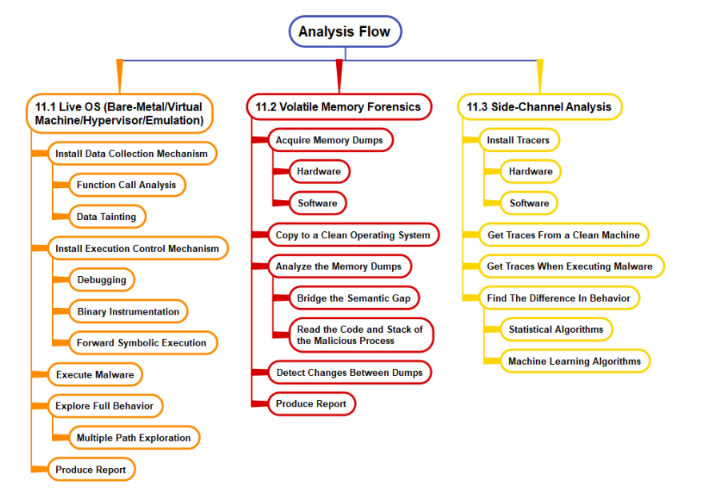
\includegraphics[width=\linewidth]{images/dynanalysis.png}
\caption{Malware analysis techniques}
\label{fig:mat}
\end{figure}

\section{Static and Dynamic Approaches}

Many different techniques can be used to dissect a malicious piece of code. However, they can be divided into two big categories: \textbf{Static Analysis} and \textbf{Dynamic Analysis}. These two are not mutually exclusive but, instead, one cannot exists without the other. Dynamic Analysis tries to fill the gaps that might arise with the static approach and is also way faster than the static one.

Although malware exists for every single operating system available this chapter and the entire thesis will be focused only on the Microsoft Windows operating system as it is the most widespread and the most targeted by malware. 

\subsection*{Static Analysis (and Its Challenges)}

\textit{Static analysis} is the process of analyzing a, possibly, malicious piece of software without running it on the machine. This is usually done with the aid of different tools, each of them specialized in performing a very specific task to extract as much information as possible from the executable. 

This type of analysis can sometimes be challenging especially when there are few information available about the target system for the malware. AS a matter of fact if the analysis is not carried out with the right tools or configurations it can lead to False Positives or False Negatives. There is therefore the need to use different techniques to first identify the Instruction Set Architecture and then run the appropriate analysis tools. Fill this gap~\cite{Nicolao2018ELISAEI}~\cite{kairajarvi2019usable}~\cite{10.1145/3374664.3375742}.

In order to fully understand how static analysis works it is important to introduce first the file format which characterizes windows binaries: Portable Executable or PE. This type of file is logically divided into 2 main parts: header and sections as it can be seen in Figure~\ref{fig:pe}.

\begin{figure}[ht]
\centering
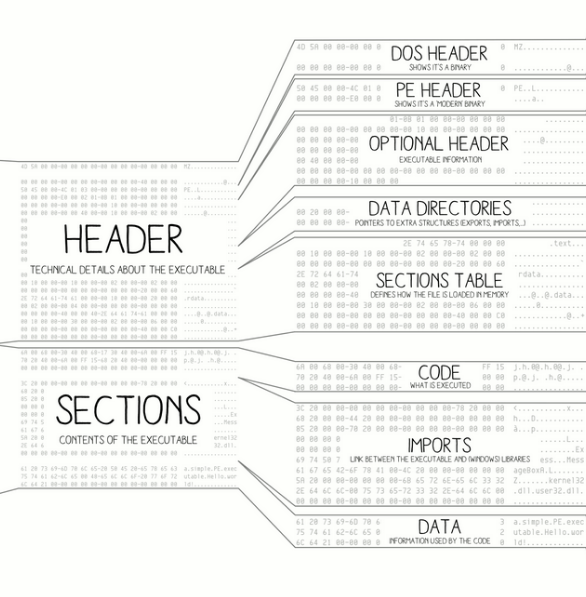
\includegraphics[width=\linewidth]{images/pediv.png}
\caption{Portable Executable format structure. From \url{corkami.com}}
\label{fig:pe}
\end{figure}

The header section contains technical information about the file, these are used by the operating system in order to properly load the executable in memory and to run it. Some of the relevant information that can be found in this part are: the machine architecture, the number of sections as well as the address, size and name of the sections.

The sections part contains the code of the executable in a format that can be interpreted by the processor as well as the libraries imported, the functions imported from such libraries and the constant strings used in the code.

Static Analysis is performed on both parts of this file. The names of the sections are particularly useful when identifying potential malware. For example, some packers change the name of the sections of the target executable inside its header. Packers are specialized programs used to obfuscate and encrypt the real code of the malware.

 On the other hand, malicious IPs and domains used for beaconing can be found in the data sections if they are saved in clear and directly used in the malware.  

Another big part of Static Analysis however consists of reading the compiled code of the malware and trying to understand what it is trying to achieve. This can be done using a disassembler which is a program that allows the user to ``reassemble'' binary machine code and convert it into a human-readable one. Such process can be further improved with the use of a decompiler, this software tries to bring a higher level of abstraction into the reverse engineering process by decompiling machine code into a pseudo-language, often similar to C, thus reducing the effort required by the analyst to interpret machine code.

This kind of analysis is usually very time-consuming and requires a deep understanding of the underlying architecture of the processor. Moreover, the malware author can use different techniques to modify the compiled code making it harder to reverse engineer or even to trick the analyst into believing that the code has different capabilities than the real ones. These techniques are commonly referred to as \textbf{Obfuscation} however many different techniques are used to hide malware capabilities: \textit{Encryption, Packing, Obfuscation, Polymorphism, Metamorphism}.~\cite{Ye2017ASO}

\textit{Encryption} and \textit{Obfuscation} are similar techniques used to hide pieces of the malicious code not only from the analyst but also from antivirus software. At low level often \textit{Encryption} consists of performing a \textit{XOR} operation on a defined portion of memory while \textit{Obfuscation} involves masquerading API calls and split strings in the code in order to make it harder to understand the real behavior of the malware.

On the other hand \textit{Packing} consists of encrypting and compressing the real code of the malware and, instead of shipping the ``real'' malicious code, the packed version will feature an unpacking stub which will take care of extracting and then running the malware directly into the memory making it harder to detect and reverse engineer.

Finally, \textit{Polymorphism} and \textit{Metamorphism} are conceptually similar. The first one involves a polymorphic engine which allows compiling the code in a non-deterministic way. This means that the output will be different at each compilation but it will still retain all the initial functionalities, this is usually achieved also with the use of encryption. \textit{Metamorphism} on the other hand is a really interesting technique through which the code of a program can be modified at run-time adding a great layer of complexity and opening the door to a dedicated category of malware.

Static Analysis is a powerful technique however for some more advanced pieces of malware it is not enough and instead it is necessary to run the malicious code in order to fully understand the capabilities and interactions with the machine.

\subsection*{Dynamic Analysis}

%\daniele{Too dry: your thesis is around dynamic analysis! Detail the different execution technologies available to date, and emphasize why whole-system emulation is important for fine-grained analysis of malware and in general for software security topics (e.g. for whole-system information flow tracking, you can cite the DECAF papers}

\textit{Dynamic analysis} is the process of running the malicious program in a controlled environment to collect as many information as possible about the behavior of a specific program. Different approaches can be taken in order to perform an effective Dynamic analysis: diffing, monitoring, tracing and debugging. The more a method is comprehensive and powerful the less it is easy to use or to implement.

\begin{itemize}
    \item \textbf{Diffing} consists of comparing the difference between a clean system and one in which the malware has run. This is usually achieved on a virtual machine using snapshots. However, this can be done also on specific parts of the system such as the windows registry or important folders. In this way it is easy to find artifacts and manipulation left on the system by the malware such as persistence through the memory. On the other hand, however, this method is not able to capture artifacts that are removed from the malware during execution.  
    
    \item \textbf{Monitoring} consists of carefully monitoring the system and capture every change on it or any network traffic that takes place after the malware is executed. In this way it is possible to have a complete overview of every action that the malware is performing on the machine. However, the data gathered in this way often have a great amount of noise and therefore needs to be filtered out and carefully examined to extract only relevant information.
    
    \item \textbf{Tracing} consists of hooking important API or System Calls in the system in order to capture important events. In this way, however, it is possible to achieve a much deeper level of details compared to System Monitoring since it is possible to monitor each external function invoked on the system. Blending in Static and Dynamic analysis and providing useful information on the execution flow of the malware as well as on the low-level interaction with the system. One of the disadvantages of this system is that it requires interpretation of the gathered information as well as to exclude data related to normal activity on the system.
    
    \item \textbf{Debugging} consists of attaching a specialized software to the malware and placing breakpoints in specific parts of the code in order to inspect the internal state of the program. This is particularly useful as it gives complete control over the execution of the malware therefore allowing to modify the internals of the machine such as processor registers, memory and so on. This approach, however, requires to deeply understand the source code of the malware in order to identify the interesting execution branches and place breakpoints correctly. Malware can easily check the presence of a debugger using a system call and can therefore change their behavior accordingly, this poses further challenges to the analyst who has to modify the environment to mask such artifact. 
    
\end{itemize}

It is of paramount importance in this phase that the machine on which the malware runs is isolated from the network. The ideal situation would be to have a real machine that can be used to run the malware and then re-imaged every time after the analysis is complete. This has some huge pitfalls in terms of performance and efficiency therefore, the best way to perform Dynamic Analysis nowadays is using a virtual machine. Such virtual machines will need to be configured in order to have proper measures in place to avoid external communication and stop the malicious program from spreading to other machines in the network. 

Different level of analysis requires a different amount of visibility and interaction with the environment. In particular, in order to extract as much information as possible from an analyzed system, it is necessary to have complete control of every single component. For this reason Virtual Machines created on a Full System Emulation environment are particularly suited for the job as they allow for fine-grained control over the simulation. In such a system, it is possible to place custom pieces of code at very specific points of the simulated hardware. This practice, called instrumentation, allows the analyst to instrument not only the malware but also the environment itself, in this way the analysis can be performed at different levels making it more efficient, rich and also completely transparent for the malware.

For example, Whole System Emulation allows the user to interact and control directly the emulated CPU making it easy to extract opcodes and make changes to a live program from outside the system. This is particularly important when analyzing malware that attempt to detect and evade the analysis environment. 

Some more advanced Dynamic Analysis techniques have been analyzed in~\cite{10.1145/2089125.2089126}. This survey proposes 3 different types of advanced techniques that can be used in an automated way to aid malware analysis:

\begin{itemize}
    \item \textbf{Function Call Monitoring} consists in placing a hooking mechanism in interesting functions in order to analyze them and possibly manipulate the results. These can be System Calls as well as API Calls. This method has many different pitfalls and depending on the implementation used. A brief analysis of the methods can be seen in the next pharagraph.
    \item \textbf{Function Parameter Analysis} consists in analyzing the values passed to the various function calls by the malware sample. A use case for this can be to understand the interaction with the system without having to monitor it. As a matter of fact, communication with the Operating System takes place through system calls which can be intercepted and further analyzed. A common analysis method to correlate how different function calls interact is called Taint Analysis and consists of marking a specific data and tracing its movement through the execution.
    \item \textbf{Information Flow Tracking} this is similar to the previously described method but, instead of focusing only on function parameters, it aims at tracing precise information. As a matter of fact, Taint Analysis can be applied not only to function parameters but also to functions themselves, pointers, memory regions, single strings and many other objects. 
\end{itemize}

Different techniques can be used to perform Function Call Monitoring, the most relevant are Dynamic Binary Instrumentation (DBI) and Virtual Machine Introspection (VMI).

DBI can be defined as follows:

\textit{``A DBI system is an execution run-time running in user space for process-level virtualization. An un-modified compiled program executes within the runtime as would happen in a native execution, with introspection and execution control capabilities accessible to its users in a programmatic way.''}~\cite{dbi}

While a definition of VMI is given in~\cite{7299979}: 

\textit{``Virtual Machine Introspection(VMI) consists in monitoring Virtual Machines (VMs) from the hypervisor level or from a privileged VM in order to inspect states and activities of Operating Systems running inside them (called guest OSes)''}~\cite{7299979}


DBI is an advanced solution that can be used to deeply inspect the malware. It allows to insert custom probes or user defined routines in a running program. This allows both to monitor and alter the execution. However, such system can be easily detected by malware as it introduces clearly visible artifacts in the system as described for example in~\cite{bruening}~\cite{corsec}~\cite{bots16}. Although some systems have been proposed in ~\cite{10.1007/978-3-319-60876-1_4} to avoid such detection, DBI remains a highly invasive technique. On the other hand, VMI allows to carry out the same kind of analysis but from a different prospective. As a matter of fact, while with DBI routines are inserted in the space of a running program, with VMI techniques it is possible to observe the entire state of the virtual machine and then place routines at different level. Since with VMI there is complete control over the system it is possible to insert such analysis sequences in a completely transparent way with respect to the malware. On the other hand, due to this further abstraction provided by VMI, it is not possible to use native system constructs and system calls from inside such analysis routines as it can be done natively with DBI. As clearly stated in~\cite{10.5555/874075.876409}:

\textit{``Writing useful analysis tools in this domain is challenging because of the semantic gap between virtual machine events and the corresponding operating system actions. The analysis tool may have to duplicate some operating system functionality to distill the log into useful information.}~\cite{10.5555/874075.876409}

Many different approaches have been proposed in the recent years to try and bridge the semantic gap explained above, Virtuoso\cite{5958036} is an example of recent framework specifically aimed to this. Virtuoso utilises a particular approach consistig in automatically crating abstraction for events observed in the introspected system. A brief description of the working mechanism can be found in the paper:

\textit{``Virtuoso creates introspection tools for an operating system by converting in-guest programs that query public APIs into out-of-guest programs that reproduce the behavior of the in-guest utilities. This is done in three phases: a training phase, in which an in-guest program that computes the desired information is run a number of times, and a record of each execution is saved; an analysis phase, which extracts just the instructions involved in computing the data required for the introspection, merges the traces into a single program, and translates that program into one that can be executed from outside the virtual machine; and finally a runtime phase, in which the generated program is used to introspect on a running virtual machine.''}\cite{5958036}

\medskip
Dynamic as well as Static Analysis must be carried out by a single person which must dedicate many hours to deeply understanding and dissecting the malicious code. Although this is highly reliable and produces a great amount of information it is not scalable or efficient. For this reason, some ad-hoc solutions to carry out an initial triage have been developed. Such solutions are dedicated virtual machines, called sandbox, inside which it is possible to safely run the malware. The analysis framework will then take care of performing different types of analysis, from network traffic to registry interaction, in order to determine the nature of the executable. This is often referred to as automatic malware analysis, some solutions will simply produce a report detailing all the actions performed on a system by a specific executable. Others will try to perform some further analysis on such data in order to understand if the binary is malicious or not. Nowadays the most common sandboxes are: cuckoo\footnote{\url{https://cuckoosandbox.org/}}, joe sandbox \footnote{\url{https://www.joesandbox.com/}}, any.run\footnote{\url{any.run}} and VMRay \footnote{\url{https://www.vmray.com/}}. Most of these solutions provide web-based user interfaces through which it is possible to submit samples to the underlying system and retrieve the results of the analysis. 

In most cases, the best analysis technique is a combination of the Static and Dynamic ones. As a matter of fact debuggers are often used to unpack malware by setting breakpoints in the code and running it in a controlled environment until the real malware is extracted and loaded into memory, the resulting piece of code can then be dumped to disk and statically analyzed.

\subsection*{Other Possible Approaches}

The two described method above requires that the analyst has acquired the executable of the malware and is able to dissect it on disk or run it in a safe environment. There are however some cases in which this is not possible, an example is file-less malware where the entire malicious code resides in memory and never touches the disk. In this case the analysis must be carried out on a snapshot of the system. 

There are two different approaches when creating a snapshot of the memory: one is dumping the entire content of the ram on disk and then carry out the analysis on it. This has many advantages as it will contain, most likely, all the information needed to carry out a complete analysis. Moreover, this will include also kernel structures that will be fundamental when trying to reconstruct the execution of the malware in memory. Moreover, from such memory dump, it is possible to select the memory region in which the malicious code resides and perform a Static analysis on it. The disadvantage of this technique is that the dump file will be of the same size of the ram and only a small portion of it will be really useful for the analysis making it harder to handle and slowing down some analysis tools. 

The volatility framework\footnote{\url{https://github.com/volatilityfoundation/volatility}} is the state of the art for this kind of analysis, it implements many different plugins that are capable of performing different types of analysis on a RAM dump file. 

The second approach consists of creating a Full Memory Dump of a single program. Such file, as opposed to the above mentioned one, will contain only the portion of memory reserved to the specified executable. In this way, some information about the system, such as the kernel structures, is lost but the produced file will be much smaller. This portion of memory, most of the time, will contain enough information to carry out full malware analysis of the malicious code. 

In addition to the above there other solutions that can be used to aid malware investigation. One can think about substituting the virtual machine with a containerized solution such as docker. As a matter of fact, this is efficiently used for some kind of analysis. In ~\cite{9042158} it has been detailed how docker containers can be used to build up an honeypot which is aimed at ransomware families. In the paper it is described how the system can be used as a sacrificial fake network share that can be exposed to ransomware. While the malware is running and encrypting shares on the honeypot the system will try to perform some automatic analysis which will then aid the analyst in detecting the ransomware family.

As containers use a different segregation and virtualization technique compared to virtual machines as it can be seen in Figure \ref{fig:dockvm} it is important to take some precautions when running malware inside them. 

\begin{figure}[htp]
\centering
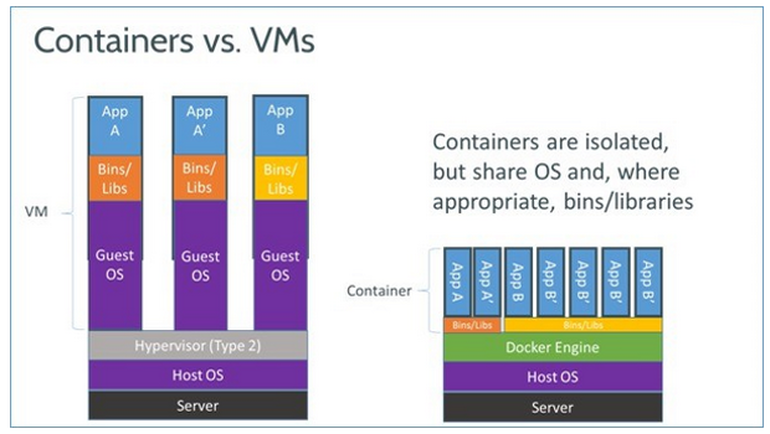
\includegraphics[width=\linewidth]{images/dockervm.png}
\caption{Differences between containers and Virtual Machines}
\label{fig:dockvm}
\end{figure}

The problem is that many of the resources are shared between containers and the host operating system meaning that there is a high risk of contamination of the host OS. In particular, it is necessary to properly configure the docker container to avoid network communication and to limit its rights. However, some problems remain as a 0-day exploit for the guest kernel can still allow for container escape. 

There are however available some further frameworks to harden the containers at kernel level. The two main ones are gVisor\footnote{\url{https://github.com/google/gvisor}} this is dedicated exactly at hardening containers by rewriting part of the Linux kernel. It is designed to limit the container access to the kernel. As stated in their github repository:

\textit{``gVisor is an application kernel for containers. It limits the host kernel surface accessible to the application while still giving the application access to all the features it expects. Unlike most kernels, gVisor does not assume or require a fixed set of physical resources; instead, it leverages existing host kernel functionality and runs as a normal process. In other words, gVisor implements Linux by way of Linux.''}

The second project is katacontainers\footnote{\url{https://katacontainers.io/}}. This project aims at fusing together Virtual Machines and containers. In particular, similarly to gVisor, katacontainers uses a custom kernel to run the containers. Such kernel is run in an isolated environment and on top of common virtualization technologies. 

In addition to these there are also other solutions like ignite\footnote{\url{https://github.com/weaveworks/ignite}} that allows to blend together containers and VMs. These are usually referred as micro Virtual Machines they provide the same performances and security as normal virtual machines but with a much lower overhead. 

Other possible approaches are based on bare metal analysis, one of them is BareBox~\cite{bbox}. Such systems try to overcome the problems associated with evasive malware and instead just run them on pysycal machines. There is, however, a huge overhead in doing this as the machine requires to be rebuilt each time a sample is run. This is because the malware can leave the virtual machine in a dirty state meaning that some artifacts from previous executions are present in the system or even that the machine is in control of the attacker. BareBox tries to overcome the problem of rebuilding the machine by providing a way to restore the state to a clean one in a way similar to VM snapshots. Live system restore is accomplished by restoring the entire physical memory of the analysis operating system from another, small operating system that runs outside of the target OS. 

\bigskip
All the mentioned solutions are general and Operating System independent. There are, however, some very specific techniques which take advantage of some features of the Linux kernel. As a matter of fact, in modern versions, it implements a feature called Extended Barkley Packet Filter. This is a method to expand the kernel in real-time. As a matter of fact, it can be used to write mini programs that can run when specific events such as disk I/O take place. These mini programs are run in a safe virtual machine in the kernel. A framework based on eBPF is tracee\footnote{\url{https://github.com/aquasecurity/tracee}}. It allows to monitor either the entire system or a single pid or container, it has many different capabilities. For example, it can be used to capture disk or memory writes which is useful for capturing process injection techniques used for fileless malware. Moreover, by intercepting syscalls allows for detailed tracing of the interaction between the OS and the sample. 

%\daniele{On Linux they also use eBPF see for instance \url{https://github.com/aquasecurity/tracee}. There are approaches for bare-metal analysis, or with instrumentation done at firmware level (check the BluePill paper, there is a nice table and discussion of other methods)}

 
\section{Evasive Malware}
\label{sec:evmal}

From an attacker perspective detecting if the malware is being analyzed can really make the difference as the more it takes for an analyst to reverse a sample the more it can stay in the wild and perform malicious actions. 

The sample has to protect itself both from Static and Dynamic analysis, as a first line of defense the malware can employ anti-dissection and anti-analysis techniques such as anti-tampering and anti-debugging sequences that break the analyst workflow. Thus forcing analysts into time consuming tasks which usually also requires to run the sample. 

As mentioned previously Dynamic Analysis takes place inside a controlled environment. Having a real computer, isolated from the network and re-imaged every time that a sample is analyzed is the best scenario but also highly inefficient. Instead, technologies such as Virtual Machines, are used nowadays to achieve the same results but with less effort, overhead and a great saving in terms of costs. A virtual machine must, however, be completely isolated from the system in order to avoid spreading the malware in the network and also exposes some ways to analyze the sample. 

For these reasons, the malware author can leverage multiple different techniques in order to fingerprint the system. In this way the malicious program can decide, based on the results of some tests if it is running on a system worth being infected or not. In particular, it is sometimes more advantageous to have a slightly higher number of false positives but avoid being easily detected, or analyzed, in the short term. 

In Figure \ref{fig:mfrm} it is possible to see how the various evasive malware behavior relates to the analysis method and environment. In particular, it can be seen how virtualized environments fail when it comes to environment fingerprinting (\textit{Detecting the Analysis Framework}). Moreover, it is possible to see how Static Analysis fails when it comes to common techniques such as code obfuscation and fileless malware.

\noindent
\begin{figure}[htp]
\centering
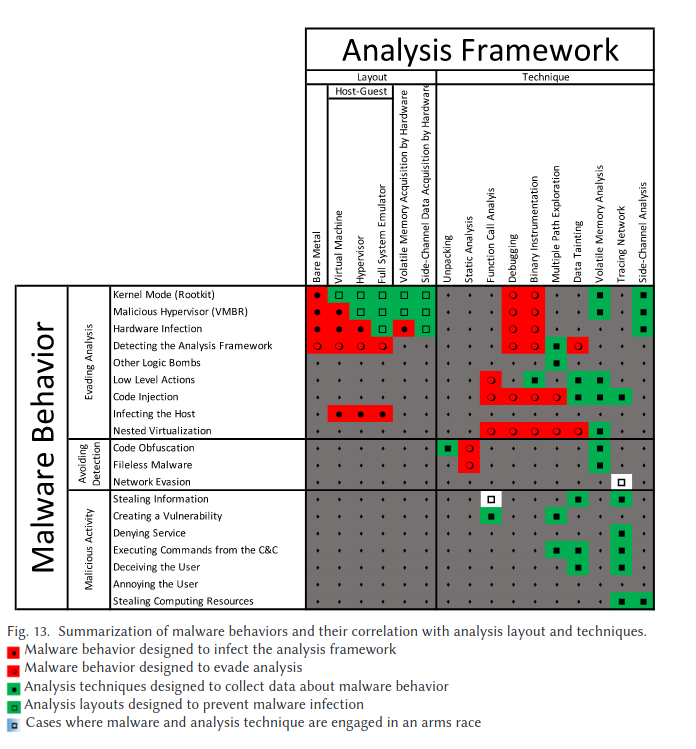
\includegraphics[width=\linewidth]{images/mal-fram.png}
\caption{Malware analysis techniques against various malware types}
\label{fig:mfrm}
\end{figure}

On the Dynamic Analysis side, the fingerprinting techniques can be broadly divided into two categories: detecting if the environment is virtualized and detecting the presence of common analysis software. 

The sequences of code dedicated to the detection of artifacts, left by the analysis system in the environment, are often referred as \textit{Red Pills}. This term was originally introduced in ~\cite{bruschi} and was limited to detecting if the CPU was emulated. It is based on the assumption that different sets of opcodes behave differently depending if they are executed inside a physical or virtualized environment. 

With the evolution of malware and analysis techniques, this term is nowadays used to indicate the generic detection of anomalies during execution. For example, red pills can be used to detect the presence of specific structures in memory that are introduced when the system is running on a hypervisor. This is typically the case of VMWare using a technique called \textit{“VMWare Magic Number”}. As a matter of fact, this Virtual Machine Manager uses a specific I/O port, called VX to communicate with the host. 

Another example of red pills are some instructions such as CPUID and RDTSC that are highly dependable on the hardware. For this reason, these are some of the best options used to detect virtual environments as described in \cite{hwvirt}.



%\daniele{Inaccurate: red pills originally detected emulators, but you should say that now you can use them to detect anomalies when executing instructions or looking up the position of specific structures in memory (see VMware artifacts) on a hypervisor or any other dynamic execution platform that is not a bare-metal machine}

The CPUID instruction\footnote{\url{https://c9x.me/x86/html/file_module_x86_id_45.html}} (shorthand for CPU IDentification) is one of the most used and interesting \textbf{Red Pills} as it can produce a good amount of details about the processor and the environment in general.

CPUID reads the input parameter from the \textit{EAX} registry and places the outputs in the \textit{EAX, EBX, ECX, EDX} registries. The length of the result is variable and therefore different registers are used according to the initial \textit{EAX} value. From a virtualization detection prospective the most interesting results are obtained by calling this instruction with the \textbf{0x1}, \textbf{0x40000000} and \textbf{0x80000000}~\cite{CPUID}. 

When calling \textit{CPUID} with 0x1 as parameter the CPU feature information are returned in \textit{ECX} and \textit{EDX}. The last 3 bits of the value in \textit{ECX} are reserved and the \nth{2} of those (i.e. the \nth{31}) bit is called Hypervisor bit, physical CPUs sets this bit to 0 while virtual ones set this bit to 1. This is a simple and fast way to detect if a program is running in a virtualized environment. 

In addition to this calling \textit{CPUID} with 0x40000000 as parameter will return the Hypervisor Brand information in \textit{EAX, ECX, EDX}. While calling \textit{CPUID 0x80000000} will return the CPU Brand information in the \textit{EAX, EBX, ECX, EDX} registries. Obviously both of the above information are set to specific values if the environment is virtualized. 

Another interesting instruction is \textit{RDTSC} \footnote{\url{https://c9x.me/x86/html/file_module_x86_id_278.html}} this is used to read the processor timestamp counter (TSC), which is a 64-bit value that stores the number of CPU cycles elapsed since the last reset. Lower bits are stored in the \textit{EDX} register while higher bits are stored in the \textit{EAX} register. The difference between two subsequent executions of this instruction on a physical CPU will be low while it will be a much higher number on virtual CPUs.

Both CPUID and RDTSC are privileged instructions, this means that they can only be executed in kernel mode, if they are executed in user mode the CPU will generate a trap. If such instructions are executed from inside a Virtual Machine a VM Exit event is generated and the control is given to the Hypervisor. Fingerprinting the time it takes to perform a VM Exit is another method used by evasive malware to detect the presence of a virtual machine. However, it must be noted that RDTSC alone is not sufficient to reliably generate a VM Exit event. As a matter of fact, this is a conditionally exiting instruction meaning that the event will be generated only under specific circumstances. On the other hand, CPUID is an unconditionally exiting instruction and therefore a VM Exit will occur each time the instruction is executed. Therefore the mechanism used by malware to fingerprint the system consists of chaining a CPUID and RDTSC instruction and comparing it to a pure RDTSC run, if the difference is above a certain threshold then the presence of a virtual machine is detected.

On the other hand \textbf{Virtualization Artifacts} are very dependant on the system employed and can be found in different places of the system. One of the most obvious artifacts is the MAC Address of the network interfaces which, by default, is set to well-known values by all the different Virtualization Software as in Figure \ref{fig:vms}.

\noindent
\begin{figure}[htp]
\centering
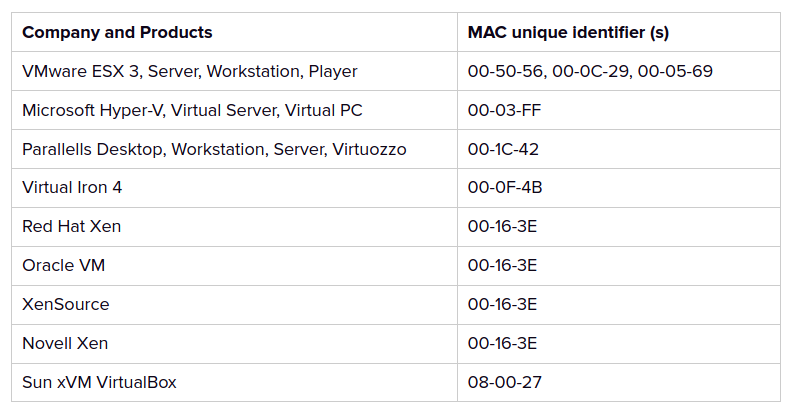
\includegraphics[width=\linewidth]{images/vms-mac-address.png}
\caption{Common VMs mac addresses \newline \url{https://www.techrepublic.com/blog/data-center/mac-address-scorecard-for-common-virtual-machine-platforms/}}
\label{fig:vms}
\end{figure}

Another common source of information for evasive malware is the windows registry, this is defined in the official documentation as a central hierarchical database used to store information that is necessary to configure the system for one or more users, applications, and hardware devices.

\textit{``The Registry contains information that Windows continually references during operation, such as profiles for each user, the applications installed on the computer and the types of documents that each can create, property sheet settings for folders and application icons, what hardware exists on the system, and the ports that are being used.''}~\cite{windocs}

The windows registry has a well-defined structure, it is organized as a tree and each node in the tree is called a \textit{key}. Each \textit{key} in the registry can contain both \textit{sub-keys} and data entries called \textit{values}. Each \textit{key} has at least 1 value called \textit{Default}. The name of each \textit{key} consists of one or more characters and is case insensitive. Sometimes the presence of a \textit{key} is sufficient for the application to store a certain setting, other times a \textit{key} will have different \textit{values} representing a piece of information. \textit{Values} can have many different types according to the information they are holding, the most common values are \lstinline{REG_BINARY, REG_DWORD} and \lstinline{REG_SZ}. 

An example of virtualization artifact related to the registry is the \textit{SystemBiosVersion} value which for VirtualBox and QEMU is as follows:
\begin{itemize}
    \item \lstinline{HARDWARE\Description\System (SystemBiosVersion) (VBOX)}
    \item \lstinline{HARDWARE\Description\System (SystemBiosVersion) (QEMU)} 
\end{itemize}

Other virtualization artifacts are system files and drivers such as, among the others:
\begin{itemize}
    \item \lstinline{system32\drivers\vmci.sys}
    \item \lstinline{system32\drivers\VBoxVideo.sys}
    \item \lstinline{system32\vboxtray.exe}
\end{itemize}

Moreover, other structures like ACPI tables, SMBIOS strings as well as Disk Size and RAM Size can be used to fingerprint the system and reveal the presence of a virtual machine. 


\section{QEMU and Emulation Artifacts}
%\daniele{give some context on QEMU, explain why relevant (you will say it in the introduction, but every chapter should be self-contained so to  speak), how dynamic binary translation behind it works, and expand the information you already have below}

As explained above at the heart of Dynamic Analysis sits a virtualization system. Such system can be based on a Hypervisor, meaning that it has minimal overhead and the analysis operating system runs directly on the hardware, or on a Full System Emulation framework. This last solution is very powerful as it allows to perform many forms of analysis in a completely transparent way. In particular, as the CPU is emulated, this means that there are intermediate steps before the code can be run on the physical CPU. Firstly the instructions for the virtual CPU needs to be translated in an architecture-independent format. Subsequently, such instructions can be further converted into ones for the real CPU. 

In all these steps it is possible to insert custom pieces of code that will allow the analyst to both trigger custom actions, called callbacks, when specific events happen on the system. Moreover, the code of the malware can be intercepted before it is run on the real CPU and modified in order to change its behavior. Since this modification happens at the (virtual) CPU level there is no way in which the malware can detect it.

The most common Full or Whole System Emulator is QEMU (Quick Emulator). It is an open-source tool capable of emulating many different CPU architectures that can be used both in Hypervisor mode and Full System Emulation mode. This last one is particularly useful in malware analysis and is at the base of many different frameworks.  

QEMU uses a sort of Just In Time (JIT) compilation process in order to translate the instruction between the emulated CPU and the real one. The translation is performed in 2 steps: first the instructions for the virtual CPU are translated in an intermediate, neutral, language through a system called Tiny Code Generator (TCG). Subsequently, TCG Opcodes are translated into instructions for the physical CPU. With such level of visibility it is possible to perform common analysis, insert breakpoints and even alter the execution flow of the program without touching the guest system. 

This transparency is one of the reasons why QEMU has a very little footprint in the guest operating system. As a matter of fact, since it does not require any custom software to be installed on the guest operating system, the ``Attack Surface'' that can be used to fingerprint the environment is greatly reduced. 

Some academic works have been proposed aiming at detecting emulated systems~\cite{hwemu}~\cite{10.1145/1572272.1572303}~\cite{184461}. These are based on the fact that the emulation introduces very specific characteristics in in the system. Timing attacks are an example, as a matter of fact emulating a system introduces an high overhead. 

As a matter of fact some of these techniques are applied by malware samples in the wild. Al-Khaser\footnote{\url{https://github.com/LordNoteworthy/al-khaser}} is a public testing suite aiming at collecting common evasive techniques. As it can be seen from the github repository the following artifacts can be used to check if the system is running on top of QEMU:

\begin{itemize}
    \item \textit{Registry Key Values:}
    \begin{itemize}
        \item \lstinline{HARDWARE\DEVICEMAP\Scsi\Scsi Port 0\Scsi Bus 0\Target Id 0\Logical Unit Id 0 (Identifier) -> (QEMU)}
    \item \lstinline{HARDWARE\Description\System (SystemBiosVersion) -> (QEMU)} 
    \end{itemize}
    
    \item \textit{Hardware Device information:}
    \begin{itemize}
        \item \lstinline{SetupAPI SetupDiEnumDeviceInfo (GUID_DEVCLASS_DISKDRIVE) -> QEMU} 
    \end{itemize}
    
    \item \textit{System Firmware Tables:}
    \begin{itemize}
        \item \lstinline{SMBIOS string checks (Qemu)}
        \item \lstinline{ACPI string checks (Qemu)}
    \end{itemize}
    
    \item \textit{Processes:}
    \begin{itemize}
        \item \lstinline{qemu-ga.exe (QEMU)}
    \end{itemize}
\end{itemize}

\textit{Registry Key Values} are used by Windows to store particular information needed to make the Operating System. The ones mentioned above are related to two hardware components, the BIOS and the Hard Disk. The custom string ``QEMU'' will end up in such values since the hardware is emulated and it will have a distinctive name. The same thing happens also with other virtualization software such as VirtualBox.

\textit{Hardware Device information} gathered through the \lstinline{SetupDiEnumDeviceInfo} function can contain interesting strings. In particular, such function can be used to retrieve information about the devices connected to the system. When queried with the \lstinline{GUID_DEVCLASS_DISKDRIVE} parameter it will return a \lstinline{SP_DEVINFO_DATA} structure for each one of them. Such structure can then be passed as parameter to the \lstinline{SetupDiGetDeviceRegistryProperty} function which will retrieve a specified Plug and Play device property, the value of such property can then be compared against known values to check if the ``QEMU'' string is present. This method is also effective against VirtualBox and VMWare.

\textit{System Firmware Tables} are particular structures loaded by specific hardware components that are available in memory on the machine. Such structures can be parsed and checked against common strings. From the official documentation SMBIOS is described as follows:

\textit{``SMBIOS offers motherboard and system vendors a standard format to present management information about their products. By extending the system firmware interface, SMBIOS can be used with management applications that use DMTF’s Common Information Model (CIM)  or another technology, such as SNMP. It eliminates the need for error-prone operations, such as probing system hardware for presence detection.''}~\cite{smbios}

While ACPI is described as:

\textit{``The Advanced Configuration and Power Interface (ACPI) specification was developed to establish industry common interfaces enabling robust operating system (OS)-directed motherboard device configuration and power management of both devices and entire systems.  ACPI is the key element in Operating System-directed configuration and Power Management (OSPM).''}~\cite{acpi}

Lastly, the only interesting \textit{Process} when it comes to QEMU is \lstinline{quemu-ga.exe}. This is called QEMU Guest Agent and is a piece of code that can be used to exchange information between the guest and the host and execute commands on the guest. This is an optional software that must be installed on the guest in order to perform very specific operations. It has a role similar to VirtualBox Guest Additions and VMWare tools which aim to provide better integration between the host and the guest. However, since this is not a critical part of QEMU, its installation on the guest system can be avoided without compromising any functionalities.  

In addition to these artifacts, hardware virtualization introduces some further red pills into the system. As explained in the previous section the CPUID instruction will return very specific strings related to the emulated CPU as well as the hypervisor bit set to 1. Moreover, the Timestamp Counter of the emulated system is based on the physical machine one. This means that, due to the fact that many translation steps are required during emulation, the RDTSC instruction can be used to detect the time needed to perform one instruction and compare it to a hard-coded bare metal threshold. 

It is clear that QEMU, compared to other systems that require the installation of additional analysis tools, is relatively transparent when it comes to evasive malware. However, due to the fact that it is widely used in analysis frameworks, malware authors have a high interest in precisely detecting it. 

\section{Environment Testing Suites}

%\daniele{Explain why they are important, how they summarize what we learn from malware in the wild (so people can't tell you that you techniques are unlikely to be effective on the average sample in the wild), and mention other sources: VMDE, SEMS, the CheckPoint collections for VM detections and anti-debug tricks, elaborate on how some techniques are general and affect multiple execution technologies (e.g. slowdown measurements vs dynamic analysis)}

The analysis environment must be carefully tested in order to discover possible artifacts that might be leveraged by the malware to avoid analysis. For this reason, different tools have been created in order to carry out as many different checks as possible and produce a detailed report that can later be used to further tweak the system.

All these tools aim to collect as many evasion techniques as possible by extracting them from malware samples observed in the wild and are regularly updated with new ones as soon as they are discovered. In this way, it is possible to test the environment against all the different fingerprinting mechanisms available to date. 

The most common testing frameworks are: 

\begin{itemize}
    \item \textbf{Paranoid Fish}\footnote{\url{https://github.com/a0rtega/pafish}} is one of the most complete tools. It employs many different techniques observed from malware in the wild to detect sandboxes and virtualization environments. Such techniques are based both on hardware characteristics such as disk or ram size as well as on specific API or System Calls. The last update of this tool was in 2016.
    
    \item \textbf{Al-Khaser}\footnote{\url{https://github.com/LordNoteworthy/al-khaser}} is the most complete and up to date tool available. This tool packs many features in order to stress test the system and run the most comprehensive analysis possible. It includes not only anti virtual machine checks but also anti-malware, anti-disassembly and dll/code injection techniques. The last update of this tool was in 2020.
        
    \item Virtual Machine Detection Enhanced (\textbf{VMDE})\footnote{\url{https://github.com/hfiref0x/VMDE}} aims to detect all types of virtual machine including whole system emulation. It relies on different detection mechanisms such as the hypervisor bit, the presence of specific objects in the system and other execution artifacts such as the presence of library modifications(hooking). The last update of this tool was in 2017.
    
    \item \textbf{SEMS}\footnote{\url{https://github.com/AlicanAkyol/sems}} is a test suite targeted at detecting Virtual machines, sandboxes as well as common analysis tools. It implements common techniques such as registry entries checking, pipes detection, files detection as well as special CPU instructions. The last update of this tool was in 2015.
    
    \item \textbf{InviZzzible}\footnote{\url{https://github.com/CheckPointSW/InviZzzible}} is a tool from CheckPoint that is based on the most common techniques. As opposed to the above ones this focuses on being future proof by giving the user the ability to add future tests in a simple way (via a json file). The last update of this tool was in 2019.
    
\end{itemize}

All the above tools will run the tests in sequence and then produce a report at the end containing the results of the various tests. It must be noted however that not all the implemented techniques are a reliable indicator of the presence of a Virtual environment. Some checks such as the disk size, number of cores or the ram size might still fail even on some moderns computers. 

Some of the analyzed techniques are general and affect multiple execution technologies, this is the case of hardware based fingerprinting. As a matter of fact such techniques can be applied to every system which is not a bare metal one. On the other hand there are some very specific detection mechanisms such as the SMBIOS strings or the presence of defined programs in the system that are really targeted to specific sandboxes or analysis environments. 

It is worth noting that similar techniques are used also by the malware to target only specific countries or devices. As a matter of fact it is increasingly common that particular malware families infects computers only if they have a specific keyboard layout. On the other hand malware can fingerprint systems and decide to infect only if they matches specific hardware requirements. 

\section{Remarks}

%\daniele{Now you should be paving the way on what you will describe in your thesis. In this chapter or in the next one you should draw also some comparison with hypervisor-based monitoring and instrumentation (DRAKVUF, Ether, etc) and explain that they do not help for some tasks that require whole-system emulation instead, or their instrumentation facilities are not flexible enough to allow some detailed analyses. If you do it in the next chapter, here you should be saying a few anticipatory things too.}

As exposed in this chapter Evasive Malware, due to their nature, are especially hard to reverse engineer and to perform Dynamic Analysis on them. In order to properly understand their capabilities it is necessary to develop systems dedicated to the analysis of such malware types. Such system can be designed in different ways, one of the simplest approach is to try to hide as many artifacts as possible. A good level of ``invisibility'' can be achieved by carefully tweaking configuration files of the various Virtual Machine Managers. For example VMWare allows to specify the values, including the hypervisor bit, that will be returned by the CPUID instruction. There are however some artifacts that might be impossible to hide and without which the Virtual Machine is not able to run. This is the case for example of drivers. 

There are different Analysis framework based on different technologies. Although some of them are based on bare-metal analysis these are beyond the scope of this thesis which is focused only on dynamic analysis performed on virtual environments.

Some of the hypervisor-based monitoring and instrumentation frameworks are DRAKVUF~\cite{lengyel2014drakvuf} and Ether~\cite{ether}, these are heavily based on virtualization support available on Intel CPUs: VT-x and Extended Page Tables (EPT). In particular it is based on the Xen Hypervisor and provides a minimal footprint on the guest system. This is an automated system which will trace the execution of a single program and provide the results gathered through Virtual Machine Introspection. Such system is however still prone to fingerprinting as it is running on a vritualized environment and timing attacks are still effective. Hiding such artifacts from the system requires deep knowledge and interaction with the Xen environment. 

Ether allows to precisely trace the execution of a sample and implements also some heuristic to detect the presence of a packed sample. On the other hand DRAKVUF allows for non interactive system analysis meaning that the interactions with the system are recorded and presented to the user. This framework also allows for syscall hooking so that the analyst can have control over the system calls performed by the malware and their results. 

Another hypervisor-based monitoring framework is rVMI\cite{rvmi}, this is based on QEMU and KVM and leverages Virtual Machine Introspection in order to act as a debugger. While the two previously mentioned systems are targeted mainly at detecting system interaction and extracting artifacts left on the system rVMI is targeted at interactive malware analysis. This framework isolates itself from the malware by placing its interactive debugging environment at hypervisor level, outside the virtual machine. By using VMI the analyst retains full control of the VM allowing to use the typical debugging features such as breakpoints and watchpoints. In addition, rVMI provides access to the entire Rekall framework feature set enabling the analyst to easily inspect the kernel and its data structures.

Lastly PyREBox~\cite{pyrebox} is another analysis framework based on QEMU that aims to aid reverse engineering by providing dynamic analysis and debugging capabilities from a different perspective. This framework allows to inspect a running QEMU VM, modify its memory or registers, and to instrument its execution, by creating simple scripts in python to automate any kind of analysis. By leveraging Virtual Machine Introspection techniques PyREBox does not require to perform any modification into the guest operating system, as it transparently retrieves information from its memory at run-time. This framework has debugging capabilities similar to rVMI and in addition it is possible to write low level callbacks in python in order to modify the state of the Virtual Machine at run time. 

On the other hand there are available multiple projects aimed at providing more visibility and control of a system by employing Whole System Emulation. 

Whole System Emulation resolves is able to hide some of the red pills described while also providing greater visibility and control over the virtualized environment. Moreover, some work has already been proposed to hide emulation artifacts in QEMU~\cite{Kang2009EmulatingEM}.

The reference analysis frameworks using QEMU in full system emulation mode are DECAF~\cite{decaf}, S$^2$E\cite{s2e} and PANDA~\cite{panda}. 

DECAF is mainly centered around taint analysis and information tracing. It is based on QEMU and has many different capabilities such as Virtual Machine Introspection and instrumentation. This last one is particularly powerful when performed on whole system emulation as it can be placed at instruction translation level minimizing overhead and intrusiveness. This framework is however is mainly based on taint analysis and, therefore, lacks some of the expansion capabilities and characteristics that are useful when performing Malware Analysis. 

S$^2$E is mainly centered on symbolic execution and finding bugs in systems or program instead of malware analysis. Although it has been designed to analyzed arbitrary pieces of software and its plugin system can be used for malware analysis this project is not regularly updated and therefore lacks some state of the art features and system updates.  

PANDA on the other hand is similarly based on QEMU. It exposes many different interfaces which allows to code custom plugins that can perform different actions. Panda focuses on providing an architecture neutral dynamic analysis platform, it does this by exposing some low level constructions and functions. These can then be used to expand the framework and create articulated analysis paths. Moreover a set of standard plugins is already provided to perform some basic analysis.

A comparison of different frameworks and their capabilities can be found in Figure~\ref{fig:frcmp}.

\begin{figure}[htp]
\centering
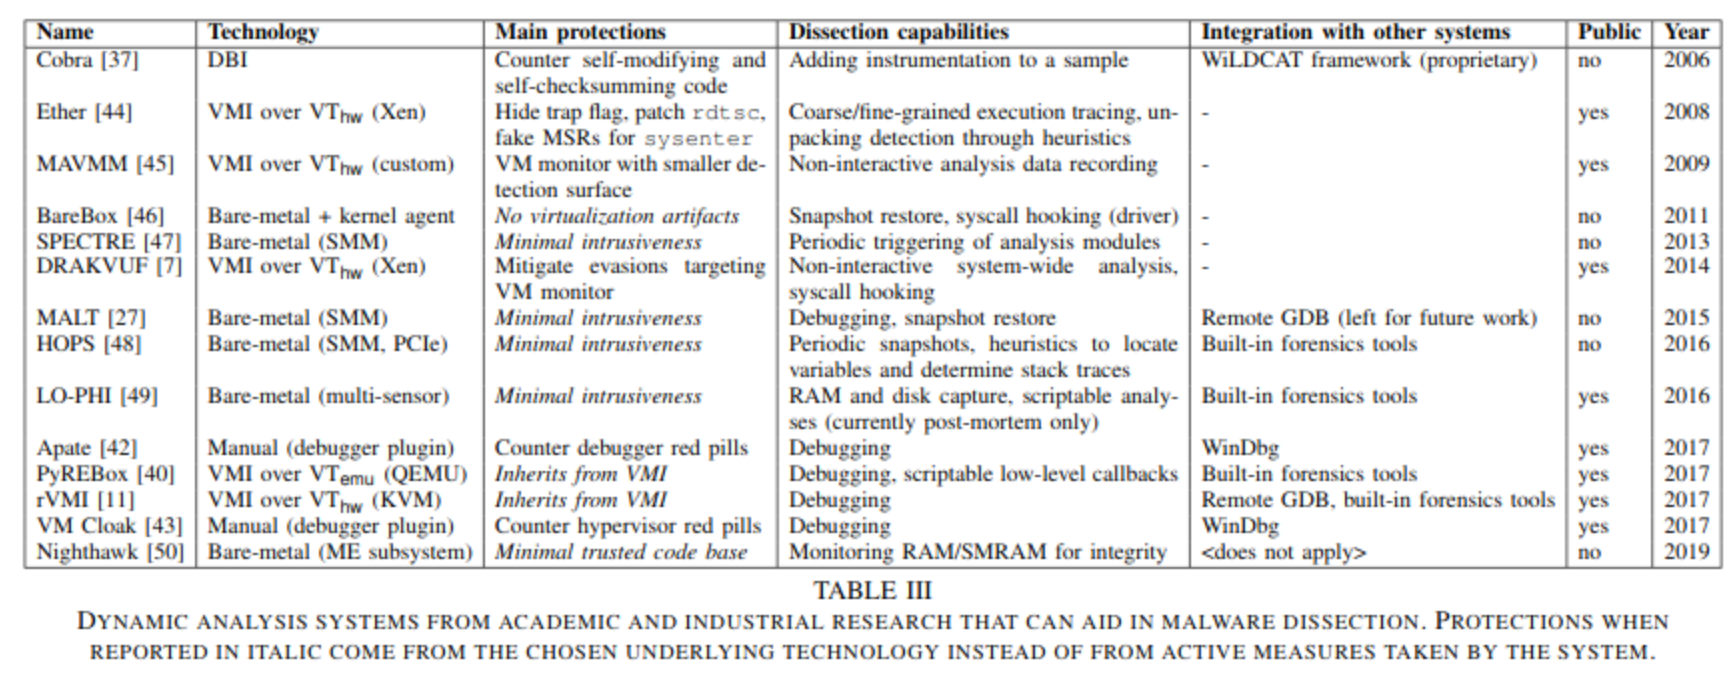
\includegraphics[width=\linewidth]{images/framcomp.png}
\caption{Comparison of different analysis frameworks~\cite{9018111}}
\label{fig:frcmp}
\end{figure}

In this thesis it has been chosen to use PANDA due to its capabilities and advantages compared to its competitors. In particular, the fact that it is based on whole system emulation and the good structures exposed, makes it a perfect candidate to chain together different plugins and perform even complex analysis. A detailed overview of all the features that PANDA provides and a small comparison to the above mentioned frameworks can be found in Chapter 4.2.